\chapter{Analyse préliminaire}

\section*{Introduction}
Dans ce chapitre, nous ferons référence aux objectifs de notre application, ce qui nous amène à identifier les possibilités du système et les besoins des utilisateurs que nous essayerons de projeter dans des diagrammes de cas d’utilisations globales.
    
\section[Spécification des besoins]{Spécification des besoins}
Dans cette partie du rapport, nous présenterons les différents acteurs du système, les besoins fonctionnels ainsi que les besoins non-fonctionnels.
\subsection[La présentation des acteurs ]{La présentation des acteurs }
Les acteurs représentent les personnes ou des composants logiciels ou matériels qui interagissent directement avec le système.\\
Dans notre projet, il y’a 4 acteurs principaux qui manipulent notre site comme l'indique la figure suivant :
\begin{itemize}
	\item Conseiller client réactif (Soit conseiller client de centre d’appel ou conseiller client de boutique)
	\item Administrateur des habilitations
	\item Administrateur
	\item Système
\end{itemize}
% TODO: \usepackage{graphicx} required
\begin{figure}[tbph]
	\centering
	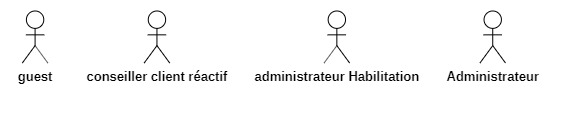
\includegraphics[width=0.7\linewidth]{img/conception/usecases/actors}
	\caption[Les acteurs de système]{Les acteurs de système}
	\label{fig:actors}
\end{figure}
\newpage
La table \ref{tab:my-table} représent les tâches de chaque acteur de notre système
\begin{table}[H]
	\resizebox{\textwidth}{!}{%
		\begin{tabular}{|l|l|}
			\hline
			\rowcolor[HTML]{C0C0C0} 
			Acteur                           & Rôle                                                                                              \\ \hline
			Conseiller client réactif        & \begin{tabular}[c]{@{}l@{}}Accès à l’application\\ Consulter les PEF au fiche client\end{tabular} \\ \hline
			Administrateur des habilitations & \begin{tabular}[c]{@{}l@{}}Accès à l'application\\ Gestion des utilisateurs\end{tabular}          \\ \hline
			Administrateur & \begin{tabular}[c]{@{}l@{}}Accès à l’application\\ Consulter les PEF au fiche client\\ Gérer toute la partie opérationnelle du projet\end{tabular} \\ \hline
			Système                          & Assure le déclenchement des tâches automatiques de l’application                                  \\ \hline
		\end{tabular}%
	}
	\captionsetup{justification=centering}
	\caption[Les tâches des acteurs de système]{Les tâches des acteurs de système}
	\label{tab:my-table}
\end{table}
\subsection[Les besoins fonctionnels]{Les besoins fonctionnels}
Notre application doit fournir un ensemble de fonctionnalités qui répondent aux exigences des acteurs. Les principales exigences fonctionnelles de notre outil peuvent être résumées comme suit le suivant:
\begin{itemize}
	\item Recevoir des rapports hebdomadaires des tests de non régression
	\item Gestion les utilisateurs
	\item Gestion les rôles
	\item Consultation des données boutiques
	\item Affectation des utilisateurs aux boutiques
	\item Gestion des catégories 
	\item Gestion des pefs
	\item Visibilité des PEF aux boutiques
	\item Simulation SRCD
	\item Consultation log
	\item Traçabilité 
\end{itemize}
\subsection[Diagramme de cas d’utilisation global]{Diagramme de cas d’utilisation global}
Dans cette sous-section, nous exposons le diagramme de cas d’utilisation global qui permet de donner donner une vision globale du comportement fonctionnel de notre système.\\
La figure \ref{fig:usecasediagram-global} représente le diagramme de cas d’utilisation global.
\begin{figure}[H]
	\centering
	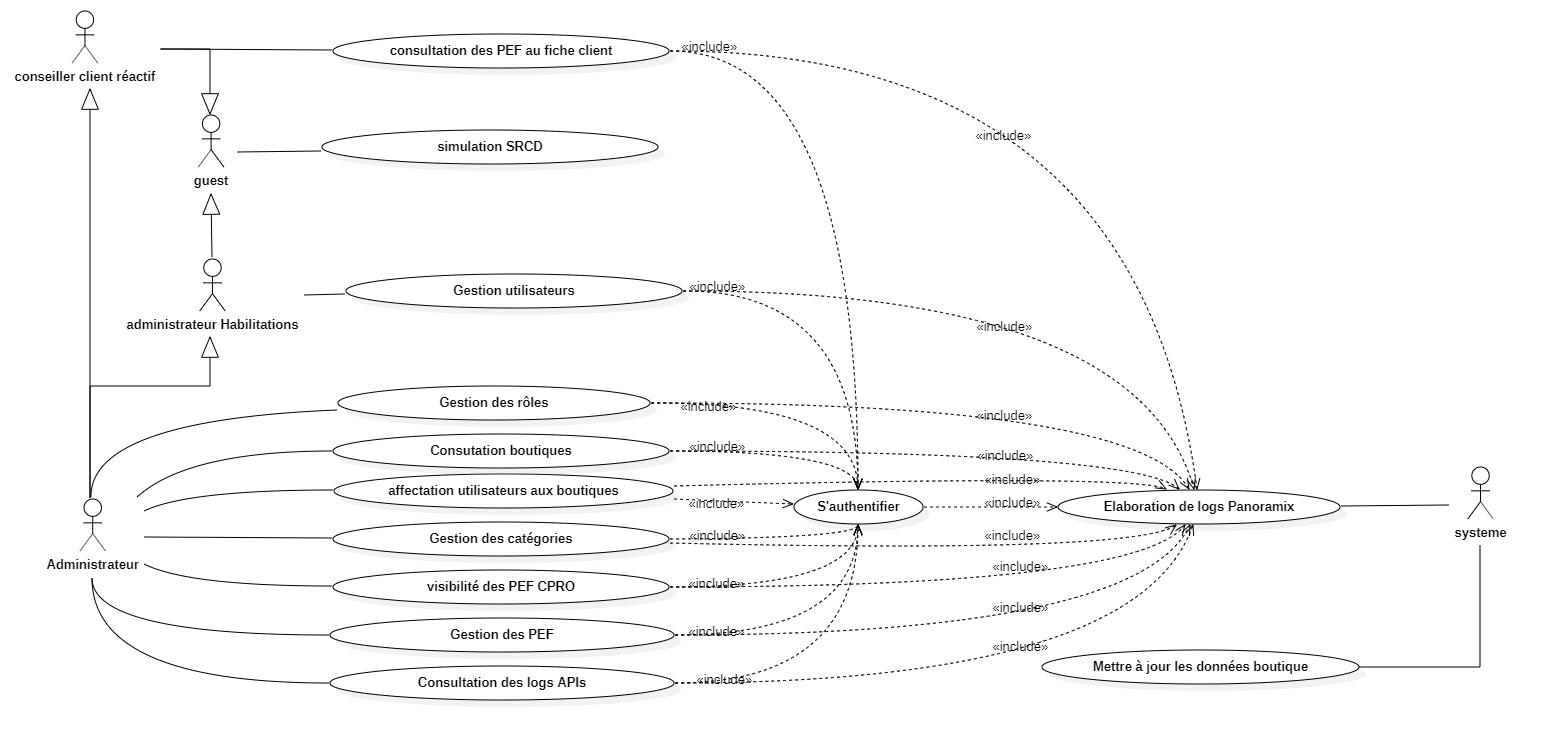
\includegraphics[width=1\linewidth]{img/conception/usecases/UseCaseDiagram-global}
	\caption[Diagramme de cas d'utilisation générale]{Diagramme de cas d'utilisation générale}
	\label{fig:usecasediagram-global}
\end{figure}
\subsection[Les besoins non fonctionnels]{Les besoins non fonctionnels}
Outre des besoins fonctionnels, le futur système doit également répondre aux contraintes suivantes :
\begin{itemize}
	\item \textbf{La rapidité de traitement :} Compte tenu du grand nombre de transactions par jour, le temps de traitement doit être le plus proche possible du temps réel.
	\item \textbf{La performance :} Nous utilisons les performances pour spécifier la durée pendant laquelle le système répond aux demandes d'entrée. Ce terme fait référence à la vitesse à laquelle le système effectue le traitement.
	\item \textbf{La disponibilité :} L'application devrait être opérationnelle d'une façon continue car l’utilisateur peut faire des réservations à tout moment. Le système doit être en permanence à la disposition de ses utilisateurs.
	\item \textbf{Ergonomie et Simplicité :} Cette fonctionnalité permet à l’utilisateur d’être à l’aise lors de l’utilisation ou de la consultation du site.
	\item \textbf{L’extensibilité :} Cela nous donne la possibilité d’ajouter, de modifier ou de supprimer des fonctionnalités.
	\item \textbf{Fiabilité :} Notre application doit être bien testé avant de l’héberger aux clients à fin d’éviter les éventuels des bugs.
\end{itemize}

\section[Structure et découpage du projet]{Structure et découpage du projet}
Nous présentons, dans la suite, les différents intervenants dans notre projet ainsi que le cycle de vie de la méthode Scrum et nous finissons par la présentation de notre product backlog.
\subsection[Identification des rôles dans l’équipe SCRUM]{Identification des rôles dans l’équipe SCRUM}
Dans un projet SCRUM, l’équipe a un rôle fondamental : elle permet d’optimiser la productivité et la flexibilité. En effet, elle doit être auto organisée et multifonctionnelle.\\
Cette méthode agile intègre généralement la participation de plusieurs acteurs, dans notre contexte nous avons le "Product owner" qui  est la personne qui porte la vision du produit à réaliser, et qui est responsable de la gestion du "backlog produit" et de l'interaction avec l'équipe de développement. Il est généralement un expert du domaine métier du projet. Mme « Nisrine ZIADIA » est le "Product owner" et Mme « Meriem OUEDERNI »  joue le rôle de "Product owner Proxi. ".\\
Le "Scrum master" est la personne qui doit maîtriser la méthodologie SCRUM et s’assurer qu'elle est bien comprise et appliquée. M. « Mohamed Aymen FEKIRI » est le "Scrum master".\\
L'équipe traduit les exigences en fonctionnalités pour obtenir des incréments utilisables et livrables à la fin de chaque itération. Notre équipe est pluridisciplinaire et auto-organisée. Cette dernière comporte un seul stagiaire, moi-même, Lassad KEFI, étudiant en Ingénierie des systèmes intelligents à L'Ecole Nationale des Ingénieurs de Carthage, qui joue le rôle d’un développeur au sein de l’équipe Panoramix.
\subsection[Planification d’un projet par Scrum]{Planification d’un projet par Scrum}
Pour appliquer correctement SCRUM, il faut comprendre le cycle de vie d’un sprint pendant un processus SCRUM. Le processus, illustré dans la figure \ref{fig:scrum}, est décrit ci-dessous: 
\begin{enumerate}[label=\arabic*.]
	\item le Product owner crée le "product backlog" en identifiant et priorisant les user stories.
	\item Pendant la planification du sprint, l’équipe choisit un ensemble de " user stories " les plus prioritaires à partir du "product backlog" pour construire le sprint Backlog. 
	\item L’équipe implémente les "users stories " pendant une période qui dure de 2 à 4 semaines. 
	\item Durant le sprint, l’équipe se réunit chaque jour, "Daily Scrum", pour synchroniser les tâches. 
	\item A la fin du sprint, le travail doit être achevé pour faire une démonstration au client. 
	\item Le sprint est clôturé par un "sprint review" pour discuter les prochaines étapes du projet et par un "sprint rétrospective" pour parler des manières à appliquer pour rendre l’équipe plus productive.
\end{enumerate}
\begin{figure}[H]
	\centering
	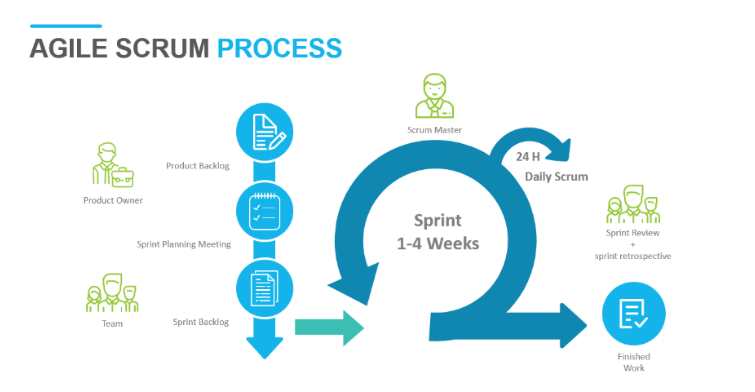
\includegraphics[width=0.9\linewidth]{img/scrum}
	\caption[Description de processus SCRUM]{Description de processus SCRUM}
	\label{fig:scrum}
\end{figure}
\subsection[Le Product Backlog du produit]{Le Product Backlog du produit}
Le backlog est élaboré avant le lancement des sprints, dans la phase de préparation. Il est utilisé pour la planification de la release, puis à chaque sprint, lors de la réunion de planification du sprint pour décider du sous-ensemble d’éléments. Les éléments y sont classés par priorité ce qui permet de définir l’ordre de réalisation.
La table \ref{tab:product-backlog} représente notre backlog de produit :
\begin{table}[H]
	\centering
	\resizebox{\textwidth}{!}{%
		\begin{tabular}{|l|c|c|}
			\hline
			\rowcolor[HTML]{C0C0C0} 
			Backlog du Produit & \multicolumn{1}{l|}{\cellcolor[HTML]{C0C0C0}priorité} & \multicolumn{1}{l|}{\cellcolor[HTML]{C0C0C0}Estimation} \\ \hline
			Migration de l’environnement \& automatisation des tests de non régression & 1 & Haute   \\ \hline
			Gestion des utilisateurs \& des rôles                                      & 2 & Haute   \\ \hline
			Intégration de module boutique \& affectation utilisateurs aux boutiques   & 3 & Moyenne \\ \hline
			gestion catégories                                                         & 4 & Moyenne \\ \hline
			Gestion des PEF                                                            & 5 & Moyenne \\ \hline
			Simulation SRCD et consultation des logs API                               & 6 & faible  \\ \hline
			Elaboration des logs de l’application                                      & 7 & faible  \\ \hline
		\end{tabular}%
	}
    \captionsetup{justification=centering}
	\caption{Backlog de produit}
	\label{tab:product-backlog}
\end{table}

\subsection[Planification des sprints]{Planification des sprints}
Notre travail est divisé sur deux releases, le premier release contient la partie de migration de l’environnement, l’élaboration des tests de non régression et la gestion des utilisateurs et leurs rôles.\\
Le deuxième release contient la consultation des boutiques, l’affectation des utilisateurs, la gestion des pefs, la simulation SRCD et la consultation des logs.\\
Le tableau \ref{tab:plan-sprints} montre la répartition des sprints relative à notre système.
% Please add the following required packages to your document preamble:
% \usepackage{multirow}
% \usepackage[table,xcdraw]{xcolor}
% If you use beamer only pass "xcolor=table" option, i.e. \documentclass[xcolor=table]{beamer}
% \usepackage{longtable}
% Note: It may be necessary to compile the document several times to get a multi-page table to line up properly
\begin{longtable}{|c|l|l|}
	\hline
	\rowcolor[HTML]{C0C0C0} 
	\multicolumn{3}{|c|}{\cellcolor[HTML]{C0C0C0}Répartition des sprints}                                                                 \\ \hline
	\endfirsthead
	%
	\endhead
	%
	\rowcolor[HTML]{EFEFEF} 
	\multicolumn{1}{|l|}{\cellcolor[HTML]{EFEFEF}Les Releases} & Les sprints                & Les tâches                                  \\ \hline
	&                            & Migration PHP                               \\ \cline{3-3} 
	&                            & Migration SGBD                              \\ \cline{3-3} 
	&                            & Migration Framework                         \\ \cline{3-3} 
	&                            & Développement des tests de non régressions  \\ \cline{3-3} 
	& \multirow{-5}{*}{Sprint 0} & Automatisation des tests de non régressions \\ \cline{2-3} 
	&                            & Gestion des utilisateurs                    \\ \cline{3-3} 
	\multirow{-7}{*}{Release 1}                                & \multirow{-2}{*}{Sprint 1} & Gestion des rôles                           \\ \hline
	&                            & Intégration de module Boutique              \\ \cline{3-3} 
	&                            & Affectation des utilisateurs aux boutiques  \\ \cline{3-3} 
	& \multirow{-3}{*}{Sprint 2} & Simulation SRCD                             \\ \cline{2-3} 
	&                            & Gestion des catégories                      \\ \cline{3-3} 
	&                            & Gestion des pefs    \\ \cline{3-3} 
	\multirow{-6}{*}{Release 2}                                & \multirow{-3}{*}{Sprint 3} & Visibilité pef boutique                     \\ \hline
	\multicolumn{1}{|l|}{}                                     &                            & Accès aux pef via la fiche client           \\ \cline{3-3} 
	\multicolumn{1}{|l|}{}                                     &                            & Consultation des logs API                   \\ \cline{3-3} 
	\multicolumn{1}{|l|}{\multirow{-3}{*}{Release 2}} & \multirow{-3}{*}{Sprint 3} & Elaboration des logs d’application Panoramix \\ \hline
	\captionsetup{justification=centering}
	\caption{Planification des sprints}
	\label{tab:plan-sprints}\\
\end{longtable}
\section[Environnement de travail]{Environnement de travail}
Dans cette partie, nous présenterons l’environnement de travail lors de la conception et la réalisation des tâches du projet.
\subsection[Environnement matériel]{Environnement matériel}
Lors de la réalisation de notre application, nous avons utilisé un seul ordinateur dont les configurations sont les suivants :
\begin{itemize}
	\item \textbf{PC} : DELL LATITUDE E5540
	\item \textbf{Processeur} : Intel i5-4210U
	\item \textbf{RAM} : 12 Go
	\item \textbf{Système d’exploitation} : Windows 10 Entreprise	
\end{itemize}
\subsection[Environnement de développement]{Environnement de développement}
\begin{itemize}
	\item \textbf{Eclipse :} est un environnement de développement intégré (IDE) utilisé dans la programmation informatique. Il contient un espace de travail de base et un système de plugin extensible pour personnaliser l'environnement.Eclipse est principalement écrit en Java et son utilisation principale est le développement d'applications Java, mais il peut également être utilisé pour développer des applications dans d'autres langages de programmation via des plug-ins, notamment C, C++, C\#, JavaScript, PHP, Python et autres.
	\begin{figure}[H]
		\centering
		
\includegraphics[width=0.5\linewidth]{img/logos/eclipse}
		\caption[Logo Eclipse IDE]{Logo Eclipse IDE}
		\label{fig:eclipse}
	\end{figure}
	\newpage
	\item \textbf{Visual studio Code : } est un éditeur de code redéfini et optimisé pour la création et le débogage d'applications web et cloud modernes.  Visual Studio Code est gratuit et disponible sur votre plateforme favorite Linux, macOS et Windows.
	\begin{figure}[H]
		\centering
		
\includegraphics[width=0.3\linewidth]{img/logos/vscode}
		\caption[Logo Visual studio Code]{Logo Visual studio Code}
		\label{fig:vscode}
	\end{figure}
	\item \textbf{Laragon :} est un environnement de développement universel, portable, isolé, rapide et puissant pour PHP, Node.js, Python, Java, Go, Ruby. Il est rapide, léger, facile à utiliser et facile à étendre. Laragon est idéal pour construire et gérer des applications web modernes. Il est axé sur la performance, conçu autour de la stabilité, de la simplicité, de la flexibilité et de la liberté.
	\begin{figure}[H]
		\centering
		
\includegraphics[width=0.3\linewidth]{img/logos/laragon}
		\caption[Logo Laragon]{Logo Laragon}
		\label{fig:laragon}
	\end{figure}
	\item \textbf{Apache :} Un serveur HTTP créé et maintenu sur la fondation d'Apache. Jusqu'en avril 2019, c'était le serveur HTTP le plus populaire sur le World Wide Web. Il est distribué sous les termes de la licence Apache.
	\begin{figure}[H]
		\centering
		
\includegraphics[width=0.3\linewidth]{img/logos/apache}
		\caption[Logo Apache]{Logo Apache}
		\label{fig:apache}
	\end{figure}
	
	\item \textbf{MariaDB :} est un système de gestion de base de données publié sous licence GPL. Il s'agit d'une branche communautaire de MySQL: la gouvernance du projet est assurée par la Fondation MariaDB, et sa maintenance est assurée par Monty Program AB, le créateur du projet.
	\begin{figure}[H]
		\centering
		
\includegraphics[width=0.3\linewidth]{img/logos/mariadb}
		\caption[Logo MariaDB]{Logo mariaDB}
		\label{fig:mariadb}
	\end{figure}
	
	\item \textbf{HeidiSQL :} est un outil de gestion de base de données avec éditeur SQL et générateur de requêtes.  Il a été développé et optimisé pour une utilisation avec le SGBD relationnel MySQL/MariaDB.
	\begin{figure}[H]
		\centering
		
\includegraphics[width=0.08\linewidth]{img/logos/HeidiSQL}
		\caption[Logo HeidiSQL]{Logo HeidiSQL}
		\label{fig:heidisql}
	\end{figure}
\end{itemize}

\subsection[Environnement logiciel]{Environnement logiciel}
Dans cette partie, nous allons présenter les différents logiciels, framework et technologies web utilisés pour la réalisation des applications.
\begin{itemize}
	\item \textbf{SeleniumLibrary based on Python :} SeleniumLibrary est une bibliothèque de test web pour Robot Framework qui utilise l'outil Selenium en interne. SeleniumLibrary fonctionne avec Selenium 3 et 4. Elle supporte Python 2.7 ainsi que Python 3.6 ou plus récent. En plus de l'interpréteur Python normal, elle fonctionne également avec PyPy et Jython. 
	\begin{figure}[H]
		\centering
		
\includegraphics[width=0.08\linewidth]{img/logos/selenium}
		\caption[Logo SeleniumLibrary]{Logo SeleniumLibrary}
		\label{fig:selenium}
	\end{figure}

	\item \textbf{Robot Framework :} Robot Framework est un framework d'automatisation basé sur Python et extensible par mot-clé pour les tests d'acceptation, le développement piloté par les tests d'acceptation, le développement piloté par le comportement et l'automatisation des processus robotiques. Il peut être utilisé dans des environnements distribués et hétérogènes, où l'automatisation nécessite l'utilisation de différentes technologies et interfaces.	Le cadre est entouré d'un riche écosystème constitué de diverses bibliothèques et outils génériques qui sont développés dans le cadre de projets distincts. 
	\begin{figure}[H]
		\centering
		
\includegraphics[width=0.4\linewidth]{img/logos/robot-framework}
		\caption[Logo Robot Framework]{Logo Robot Framework}
		\label{fig:robot-framework}
	\end{figure}
	\item \textbf{Jenkins :} Jenkins est un outil d'intégration continue open source. Après les différends entre son auteur \textit{Kohsuke Kawaguchi} et Oracle, Jenkins devient une branche des outils Hudson. Jenkins est écrit en Java et il peut fonctionner dans un conteneur de servlet (comme Apache Tomcat), ou il peut être utiliser un serveur Web intégré en mode autonome.
	\begin{figure}[H]
		\centering
		
\includegraphics[width=0.3\linewidth]{img/logos/jenkins}
		\caption[Logo Jenkins]{Logo Jenkins}
		\label{fig:jenkins}
	\end{figure}
	\item \textbf{GeckDriver : }Proxy pour l'utilisation de clients compatibles avec le W3C WebDriver pour interagir avec les navigateurs basés sur Gecko. Ce programme fournit l'API HTTP décrite par le protocole WebDriver pour communiquer avec les navigateurs Gecko, tels que Firefox. Il traduit les appels dans le protocole Marionnette à distance en agissant comme un proxy entre les extrémités locale et distante. 
	\item \textbf{Xvfb plugin :} Xvfb ou X virtual framebuffer est un serveur d'affichage mettant en œuvre le protocole de serveur d'affichage X11. Contrairement aux autres serveurs d'affichage, Xvfb effectue toutes les opérations graphiques en mémoire sans afficher de sortie d'écran. C'est très utile si votre compilation nécessite un accès X11, par exemple pour effectuer des tests qui nécessitent une interface graphique.
	\item \textbf{Email Extension plugin : }Ce plugin vous permet de configurer tous les aspects des notifications par courrier électronique. Vous pouvez personnaliser le moment où un courriel est envoyé, qui doit le recevoir et ce que le courriel dit.
	\item \textbf{Javascript  : }est un langage de script utilisé pour créer et contrôler le contenu dynamique d'un site web, c'est-à-dire tout ce qui bouge, rafraîchit ou change de quelque manière que ce soit sur votre écran sans vous obligez à recharger manuellement une page web. Des choses comme : des graphiques animés, des diaporamas de photos, des suggestions de texte à remplir automatiquement, des formulaires interactifs.
	\begin{figure}[H]
		\centering
		
\includegraphics[width=0.13\linewidth]{img/logos/js}
		\caption[Logo Javascript]{Logo Javascript}
		\label{fig:js}
	\end{figure}
	
	\item \textbf{jQuery :}  est une bibliothèque JavaScript multiplateforme gratuite, qui a été créée pour faciliter l'écriture de scripts côté client avec du code HTML sur les pages Web.
	\begin{figure}[H]
		\centering
		
\includegraphics[width=0.3\linewidth]{img/logos/jquery}
		\caption[Logo jQuery]{Logo jQuery}
		\label{fig:jquery}
	\end{figure}
	
	\item \textbf{Axios :} Axios est un client HTTP populaire, basé sur la promesse, qui comporte une API facile à utiliser et peut être utilisé à la fois dans le navigateur et dans Node.js. Effectuer des requêtes HTTP pour récupérer ou enregistrer des données est l'une des tâches les plus courantes qu'une application JavaScript côté client devra effectuer.
	\begin{figure}[H]
		\centering
		
\includegraphics[width=0.3\linewidth]{img/logos/axios}
		\caption[Logo Axios]{Logo Axios}
		\label{fig:axios}
	\end{figure}
	
	\textbf{HTML5 :} est un langage de balisage utilisé pour structurer et présenter le contenu sur le World Wide Web. Elle est la dernière révision majeure d'HTML. HTML5 spécifie deux syntaxes pour le modèle abstrait défini par le DOM: HTML5 et XHTML5
	\begin{figure}[H]
		\centering
		
\includegraphics[width=0.2\linewidth]{img/logos/html5}
		\caption[Logo HTML5]{Logo HTML5}
		\label{fig:html5}
	\end{figure}
	
	\item \textbf{PHP :} préprocesseur hypertexte, connu sous son acronyme PHP, est un "langage de programmation" gratuit qui est principalement utilisé pour générer des pages Web dynamiques via un serveur HTTP, mais il peut également fonctionner comme n'importe quel langage interprété localement. PHP est un langage impératif orienté.
	\begin{figure}[H]
		\centering
		
\includegraphics[width=0.2\linewidth]{img/logos/php}
		\caption[Logo PHP]{Logo PHP}
		\label{fig:php}
	\end{figure}
	
	\item \textbf{Orange Framework \& Tools : } est un squelette d'application PHP/MySQL prêt-à-l'emploi. Ce framework PHP est sécurisé et équipé d'outils de sécurité pour accompagner les développements, charté et respectueux de l'identité du Groupe \#Boosted, performant et compatible avec toutes les offres d'hébergement \#12factor, souple et adapté à la construction d'interfaces REST et HTML, équipé d'outils pour accélérer les développements et gérer les spécificités d'Orange et adapté aux débutants comme aux experts.\\
	L'OFT est surtout un framework basé sur Symfony et Zend PHP, produit de réflexions sur ce qui est jugé le plus pertinent pour les projets du Groupe Orange puisqu'il est taillé selon les besoins de la communauté PHP d'Orange et qui suit les standards et réutilise les composants reconnus.
	\begin{figure}[H]
		\centering
		
\includegraphics[width=0.3\linewidth]{img/logos/oft}
		\caption{Logo Orange framework \& tools}
		\label{fig:oft}
	\end{figure}
	
	
	\item \textbf{Boosted : } est répresenté comme la bibliothèque HTML, CSS et JS d'Orange basée sur Bootstrap 4.5.0, la boîte à outils open source frontale la plus populaire au monde.
	\begin{figure}[H]
		\centering
		
\includegraphics[width=0.2\linewidth]{img/logos/boosted}
		\caption[Logo Boosted]{Logo Boosted}
		\label{fig:boosted}
	\end{figure}
\end{itemize}

\section[L'architecture de la solution]{L'architecture de la solution}
Dans cette partie, nous présenterons l'architecture logicielle et matérielle utilisée lors du développement de notre application.
\subsection[L'architecture logique]{L'architecture logique}
\subsubsection{L'architecture logique des tests de non régression}
Nous présentons dans ce qui est suit l'enchaînement des tests de non régression de notre application. La figure \ref{fig:jenkins-schema} illustre la procédure des tests.
\begin{figure}[H]
	\centering
	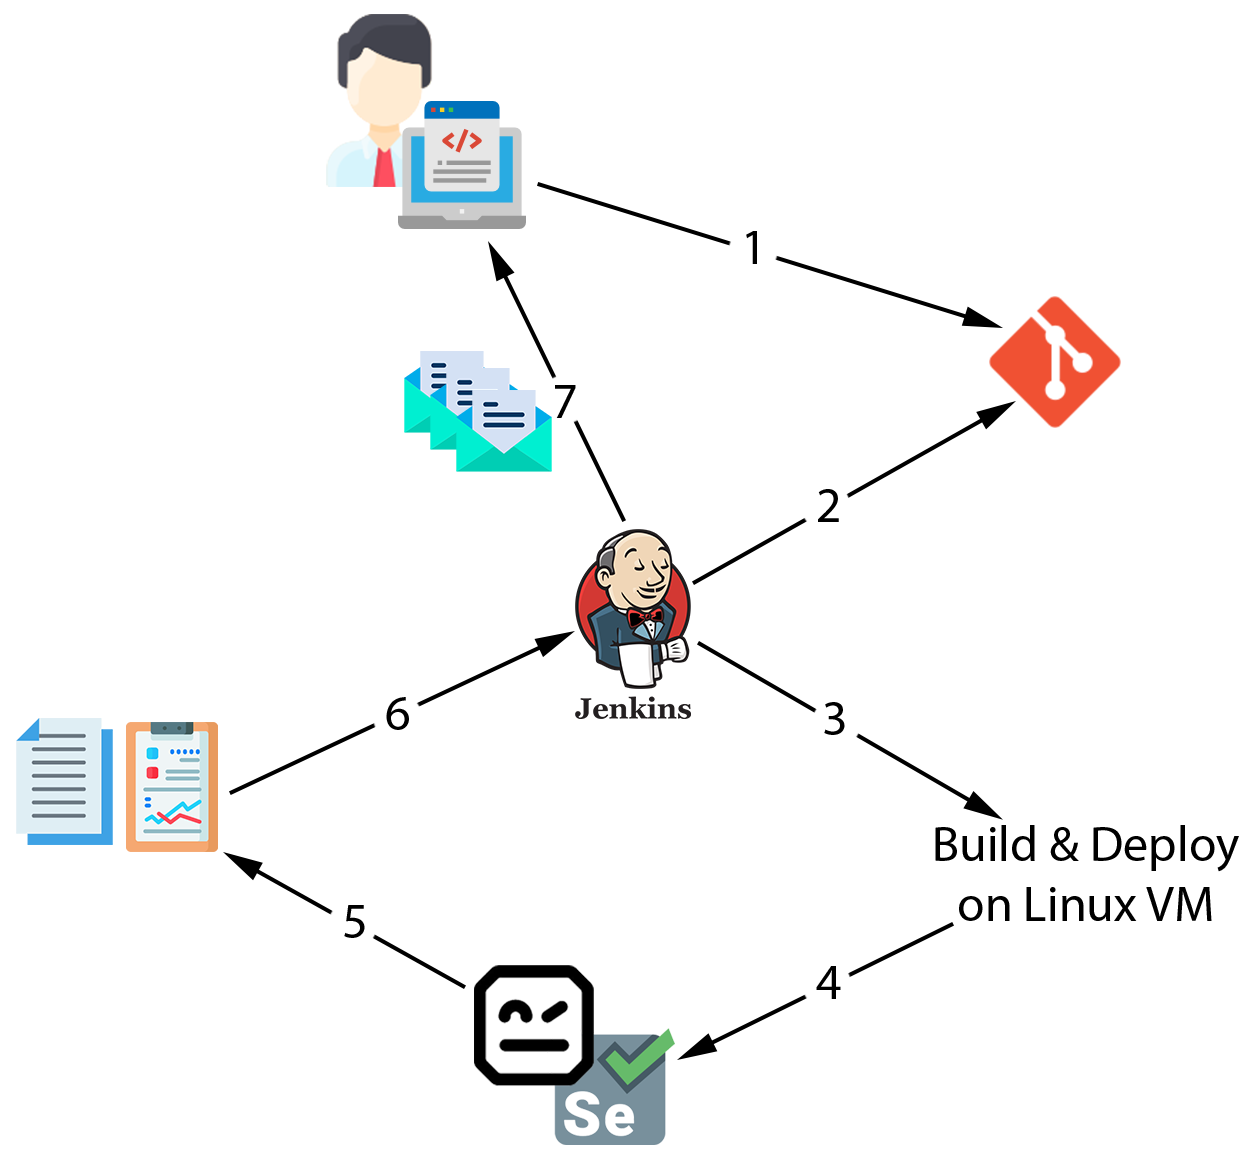
\includegraphics[width=0.5\linewidth]{img/jenkins}
	\caption[L'architecture logique des tests de non régression]{L'architecture logique des tests de non régression}
	\label{fig:jenkins-schema}
\end{figure}
\begin{enumerate}
	\item[1 -] Le développeur de l’équipe Panoramix fait un « push » de code de robot Framework vers le repo git de « Orange Forge ».
	\item[2+3 -] Jenkins va cloner ce repo dans une VM Linux et prépare l’environnement pour lancer les tests
	\item[4 -] les 54 tests de non régression s’exécutent test par test et chaque test simule un scénario d’utilisation de notre portail.
	\item[5 -] A la fin des tests, Robot Framework génère 3 fichiers dont le fichier report.html et log.html sont les plus importants :
	\begin{itemize}
		\item\textbf{ Log.html :} Les fichiers journaux contiennent des détails sur les cas de tests exécutés au format HTML. Ils ont une structure hiérarchique indiquant la suite de tests, le scénario de test et les détails des mots clés. Les fichiers journaux sont nécessaires presque à chaque fois que les résultats des tests doivent être examinés en détail. Même si les fichiers journaux contiennent également des statistiques, les rapports sont plus utiles pour obtenir une vue d'ensemble de haut niveau.
		\item \textbf{Report.html :} Les fichiers de rapport contiennent un aperçu des résultats de l'exécution des tests au format HTML. Ils contiennent des statistiques basées sur les balises et les suites de tests exécutés, ainsi qu'une liste de tous les cas de tests exécutés. Lorsque les rapports et les journaux sont générés, le rapport comporte des liens vers le fichier journal pour faciliter la navigation vers des informations plus détaillées. Il est facile de voir l'état général de l'exécution des tests à partir du rapport, car sa couleur de fond est verte, si tous les tests critiques réussissent, et rouge vif dans le cas contraire.
	\end{itemize}
	\item[6+7 -]  Jenkins récupère les fichiers générés par robot Framework et les envoyer en email vers les personnes concernés.
\end{enumerate}

\subsubsection{L'architecture logique de l’application}
Dans notre application que nous avons effectuée, nous envisageons d’utiliser une architecture 3-tiers qui sera réparti en trois couches comme suit :
\begin{itemize}
	\item\textbf{ Couche 1 (Site) :} Cette couche contient les interfaces côté utilisateurs qui interagissent souvent avec l’application Panoramix.
	\item\textbf{ Couche 2 (Serveur) : }Cette couche représente la partie traitement qui contient toutes nos APIs, cette partie sera réalisée avec Apache qui est un serveur HTTP.
	\item \textbf{Couche 3 (Base de Données) :} Cette couche représente le côté base de données de notre site qui sera une base de données MySQL.
\end{itemize}
\begin{figure}[H]
	\centering
	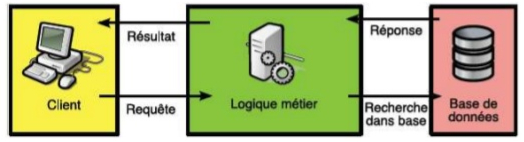
\includegraphics[width=0.7\linewidth]{img/architectures-3tiers-web}
	\caption[L'architectures 3 tiers du Web]{L'architectures 3 tiers du Web}
	\label{fig:architectures-3tiers-web}
\end{figure}

\subsection[L'architecture logicielle]{L'architecture logicielle}
\subsubsection{L'architecture logicielle des tests de non régression}
Les tests de non régression sont divisés en 3 grandes parties :
\begin{itemize}
	\item Configuration globale : un dossier qui contient un fichier de configurations globales nécessaires dans la plupart des tests
	\item Les fonctions globales : ce dossier contient un fichier des fonctions générales utilisées dans tous les tests.
	\item TestSuite :  un dossier contient tous les tests de non régression. Chaque test est divisé en 3 parties :
		\subitem • Fichier.robot : le script de test à exécuter
		\subitem • Config : est un dossier contient les configurations nécessaires pour ce test
		\subitem • Fonctions : est un dossier contient les fonctions nécessaires pour ce test
\end{itemize}
\subsubsection{L'architecture  logicielle de l’application}
L’organisation du code source est assuré par le biais du modèle MVC. Mais son rôle est principalement de segmenter la logique du code en trois parties. 
\begin{itemize}
	\item Modèle(M) : Permet de récupérer des données brutes stockées dans notre base de données.
	\item Vue(V) : Cette partie inclut juste les fichiers html et CSS mais aussi quelques boucles et conditions PHP très simples qui se focalisent sur l’affichage. 
	\item Contrôleur(C) : Ce dernier est assimilable à une passerelle entre les vues et le modèle. Il contient exclusivement que du PHP et gère notamment les droits d’accès de chaque utilisateurs. 
\end{itemize}
La figure suivante schématise l’échange d’informations entre les éléments de l’architecture MVC
\begin{figure}[H]
	\centering
	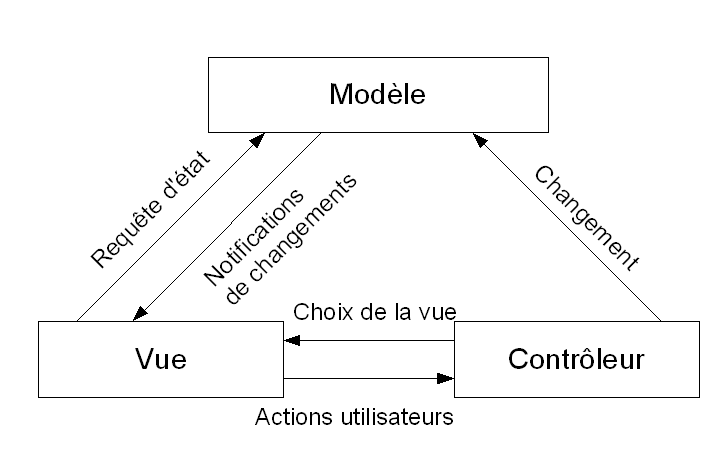
\includegraphics[width=0.7\linewidth]{img/mvc}
	\caption[L'architecture logicielle de l’application]{L'architecture logicielle de l’application}
	\label{fig:mvc}
\end{figure}

\section{Conclusion}
Dans ce chapitre, nous avons présenté les différents concepts nécessaires à la compréhension du projet. Nous avons également identifié les besoins fonctionnels, non fonctionnels ainsi que les acteurs. Par la suite nous avons réalisé une conception pour notre projet, présenté l’environnement de travail et l’architecture de la solution. Dans le chapitre suivant nous entamons le développement du premier release.